\chapter{相关工作}\label{ch:related_work}
% ------------------ Models ------------------ %
\section{生成式模型}\label{sec:generative_model}

\subsection{定义}\label{subsec:definition}
如公式~\ref{eqn:generative_cond_prob}~所示,
一个生成式模型定义了给定输入序列$X = x_1, x_2, \dots, x_n$,
输出序列$Y = y_1, y_2, \dots, y_m$的条件概率。
如公式~\ref{eqn:generative_train_objective}~所示,
模型在数据集$S$上的训练目标函数就是最大化样本的条件概率。
从定义上看,只要能估计条件概率$p(Y|X)$的模型就是生成式模型。
\begin{align}
    p(Y|X) &= p(y_1, y_2, \dots, y_m|x_1, x_2, \dots, x_n)
    \label{eqn:generative_cond_prob} \\
    \mathcal{L} &= \frac{1}{|S|} \sum_{(Y, X) \in S} \log p(Y|X)
    \label{eqn:generative_train_objective}
\end{align}

% -- RNN -- %
生成式模型需要把一个长度可变的序列$X$映射到另一个长度可变的序列$Y$,且$X$和$Y$的长度可以不相等。
循环神经网络(RNN)为这个问题提供了自然的解决方案。
RNN的基本思想是:序列由有序的元素组成,每一个时刻(Time Step)输入一个元素,同时更新内部的隐藏状态(Hidden State),然后输出一个元素。
如图~\ref{fig:RNN_unrolled}~所示,
在时间轴上展开的RNN和一般的前馈神经网络(Feed Forward Neural Networks)很相似,不过所有时刻共享一个权重矩阵$A$,
该矩阵又称为循环矩阵(Recurrent Matrix),它实现了对输入序列的编码。
\begin{figure}[H]
    \centering
    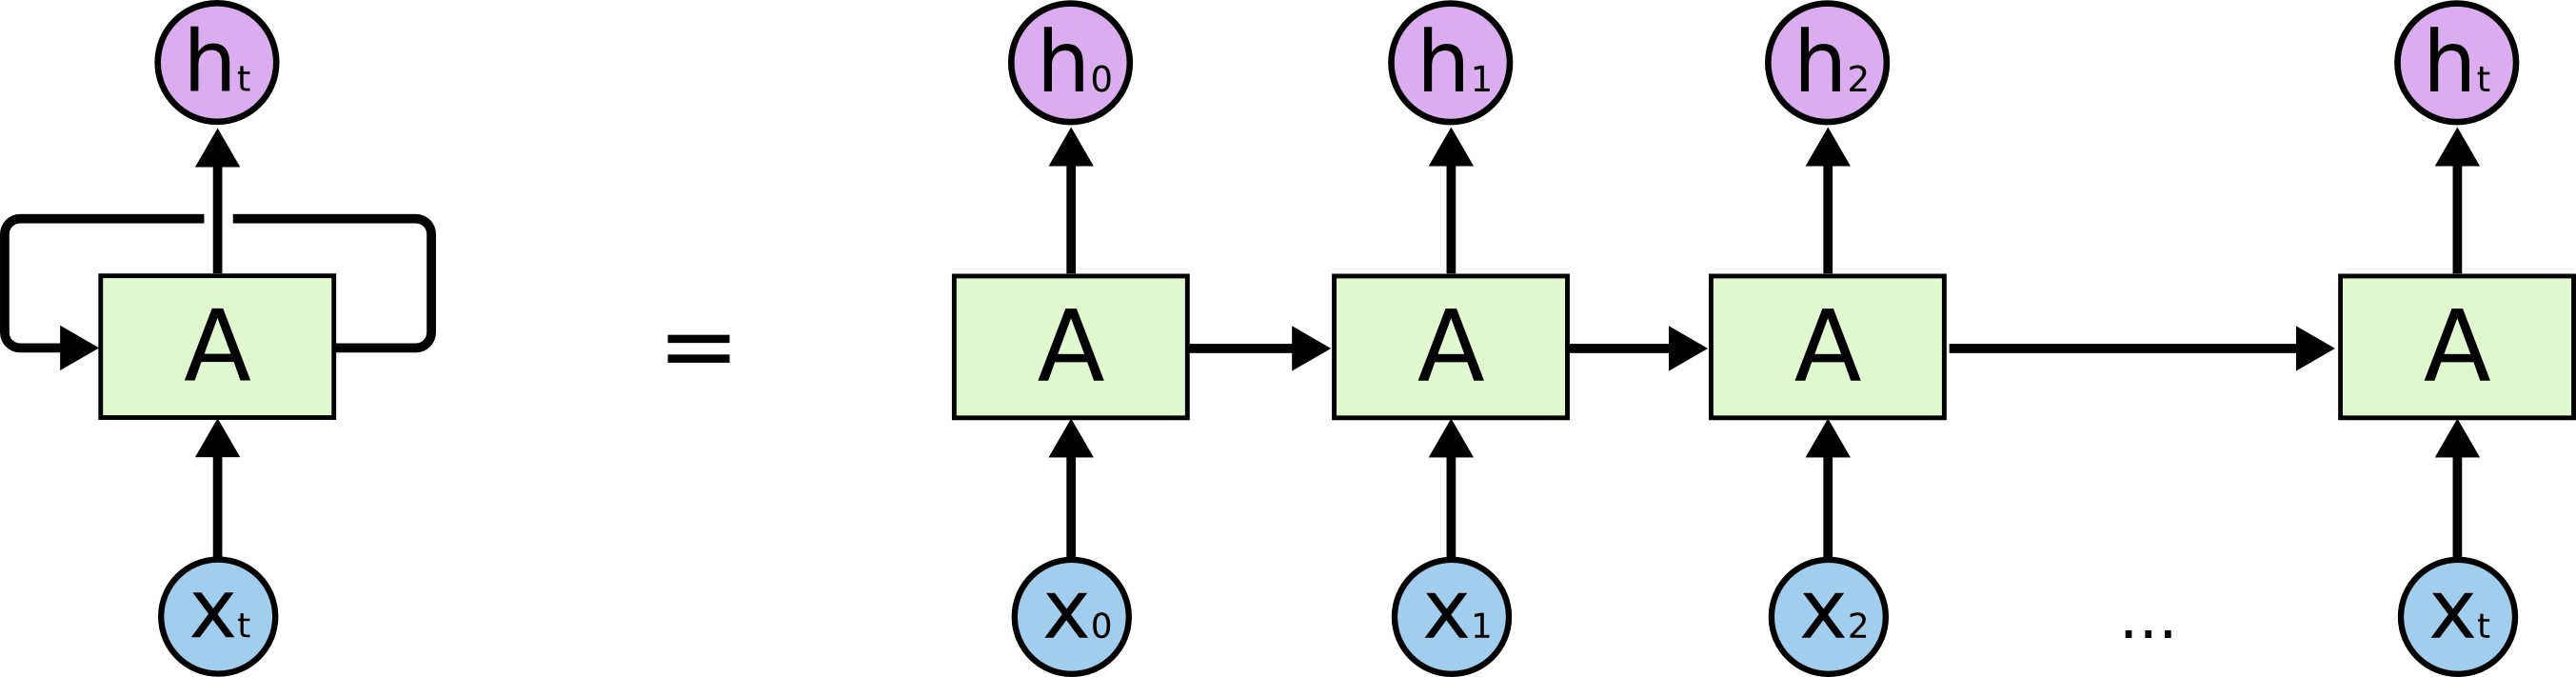
\includegraphics[width=0.6\textwidth]{figure/RNN-unrolled.png}
    \caption{在时间轴上展开的RNN}
    \label{fig:RNN_unrolled}
\end{figure}

% ------------------ RNN types ------------------ %
根据是否使用了某种门单元,RNN可分为普通RNN\upcite{RNNLM},
LSTM\upcite{LSTM}和GRU\upcite{GRU}等等。
根据是否对反向序列(Reversed Sequence)编码,
RNN可分为单向RNN(Unidirectional RNN)
和双向RNN(Bidirectional RNN)\upcite{BiRNN}。
为了更好的处理长期依赖问题,同时避免梯度消失问题的影响,一般采用LSTM或者GRU等有着特殊门单元的RNN。
为了避免梯度爆炸对模型优化的影响,一般采用梯度剪裁(Gradient~Clipping),
对超过某个阈值的梯度进行重置\upcite{GoogleChatbot}。
此外,多层RNN组成的深度循环神经网络比单层RNN有更好的性能\upcite{GoogleChatbot}。

\subsection{RNN语言模型}\label{subsec:RNNLM}
% ---------------- RNNLM ------------------ %
RNN语言模型(Recurrent Neural Network Language Model,RNNLM)
通过循环神经网络估计给定序列$X = x_1, x_2, \dots, x_n$的概率分布:
\begin{align}
    p(X) = \prod_{i=1}^{n} p(x_i|x_1, x_2, \dots, x_{i-1})
    \label{eqn:language_model_probability} \\
    p(x_i = w|x_1, x_2, \dots, x_{i-1}) = \frac{\exp{o_{tw}}}{\sum_{v=1}^V \exp{o_{tv}}}
    \label{eqn:language_model_estimation}
\end{align}

$o_t$是RNN在$t$时刻的输出向量,$V$是词汇表的大小,
一个基于普通RNN的RNN语言模型通过如下公式计算出$o_t$:
\begin{align}
    o_i &= h_i^T W_{out} \\
    h_i &= \sigma \left( x_i^T W_{in} + h_{i-1}^T W_{hh} \right)
\end{align}

$W_{in}$是输入矩阵,$W_{out}$是输出矩阵,$W_{hh}$是循环矩阵,
$\sigma$是激活函数。
RNN语言模型在训练时最大化训练集上的句子的对数概率:
\begin{align}
    \mathcal{L(X)} = \sum_{i=1}^n \log p(x_i|x_1, x_2, \dots, x_{i-1})
\end{align}

\subsection{Seq2Seq框架}\label{subsec:Seq2Seq}
% ------------------ Seq2Seq ------------------ %
如图~\ref{fig:Seq2Seq}~所示,
Seq2Seq框架使用两个具有独立参数的RNN分别作为编码器和解码器。
首先,编码器把输入序列$X$编码成一个定长向量$v$。
该向量又称为思考向量(Though Vector),
是编码器在最后一个时刻$t_{n}$的隐藏状态(Last Hidden State)。
接着,解码器以$v$为初始隐藏状态(Initial Hidden State)生成输出序列。
\begin{figure}[H]
    \centering
    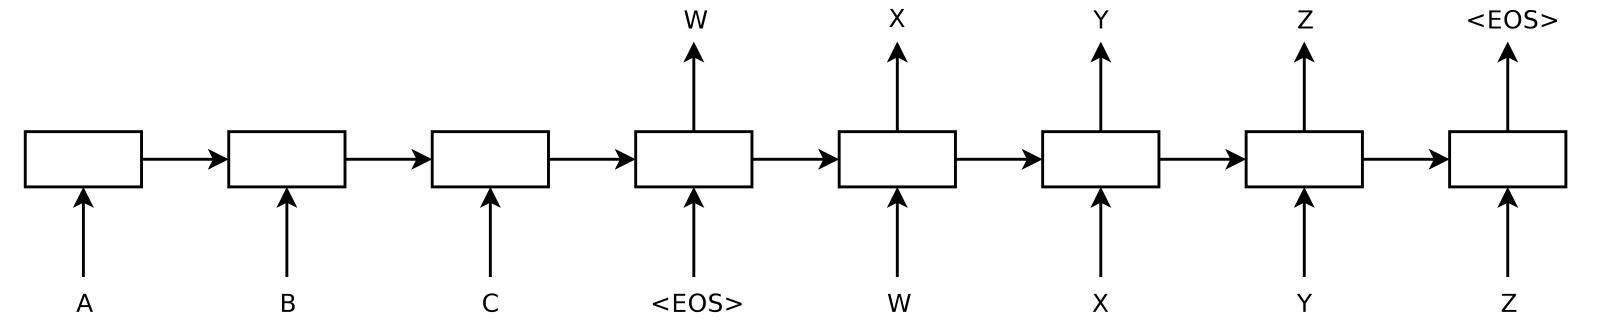
\includegraphics[width=0.8\textwidth]{figure/Seq2Seq.png}
    \caption{Seq2Seq框架图\upcite{Seq2Seq}}
    \label{fig:Seq2Seq}
\end{figure}

通过先把输入序列$X$变换成某种压缩编码$v$,
再把$v$还原为另一个序列$Y$,
Seq2Seq对公式~\ref{eqn:generative_cond_prob}~作了如下转化:
\begin{align}
    h_i &= f(x_i ,h_{i-1}), v = h_n \\
    p(y_1, y_2, \dots, y_m|x_1, x_2, \dots, x_n) &=
    \prod_{i=1}^m p(y_i|v, y_1, y_2, \dots, y_{i-1})
\end{align}

$h_n$是编码器的最后一个时刻的隐藏状态,$f$是编码器RNN所使用的门单元的抽象表示。
编码器和解码器以同一个目标函数一起训练。

为了更好的处理长序列,
Seq2Seq一般引入注意力机制(Attention Mechanism)
\upcite{JointTransAlign,EffectiveAttention},
使输入序列的信息不必全部通过固定长度的向量$v$传递。
该机制使解码器能自动关注和当前输出最相关的输入部分,
实现输入序列与输出序列的对自动对齐(Automatic Alignment)。

% ------------------ Decoding ------------------ %
\subsection{解码算法}\label{subsec:decode}
从生成式模型定义的概率分布中产生输出序列的过程称为解码(Decoding)。
生成式模型虽然可以估计任意输入输出对$(X, Y)$的条件概率$p(Y|X)$,
但是对于任意给定输入$X$,所有可能的输出$Y$的数量过于庞大,不可能枚举所有的$Y$并求其中概率最大者。
所以在解码过程中,需要使用某种启发式搜索算法从所有可能的输出中产生一个近似最优解,
这些算法又称为解码算法。
最简单的解码算法是贪心搜索(Greedy Search),
如公式~\ref{eqn:greedy_search}~所示,该算法在每一时刻都选择使当前句子的条件概率最大的单词。
因为公式~\ref{eqn:greedy_search}~中的各个$y_i$都不是独立的,
而受之前输出的单词的影响,所以贪心搜索不能保证得到条件概率最大的输出序列。
\begin{align}
    y_i = \argmax_{w \in V} p(w|y_1, y_2, \dots, y_{i-1}, X)
    \label{eqn:greedy_search}
\end{align}

如公式~\ref{eqn:random_sampling}~所示,随机取样(Random Sampling)
在每一时刻都按照模型输出的单词的概率分布随机选取一个单词。
随机取样能在一定程度上避免单调响应的问题\upcite{HRED},
然而在更多时候,它会导致输出中出现语法错误\upcite{DiverseBeam}。
\begin{align}
    p(y_i = w) = p(w|y_1, y_2, \dots, y_{i-1}, X), w \in V
    \label{eqn:random_sampling}
\end{align}

集束搜索(Beam Search)是一种标准的解码算法,
它在生成整个输出的过程中维护一个大小为$B$的列表,称为集束(Beam)。
算法开始时,集束初始化为模型生成的$B$个概率最高的单词。
算法的循环不变式如下:
每一次迭代开始前,集束中都有$B$个部分生成的句子,它们称为候选$Y_c$。
每次迭代,算法对集束中的每一个候选都生成$B$个概率最大的下一个单词$w_{i+1, c}$,
从而形成$B \times B$个部分生成的句子,
它们称为扩展的候选集。
迭代结束时,算法只保留扩展的候选集中前$B$个概率最大的句子。
迭代不断进行直到某些候选中产生了句子结束符号(End-of-Sentence,EOS),
此时算法结束并将这些完成的句子作为输出。
本质上,集束搜索是一种队列长度有限的宽度优先搜索
(Breath First Search)。

% -- Diverse Beam -- %
为了增加模型输出的多样性,学者们提出了许多改进的解码算法。
Li等人提出了Diverse Beam算法\upcite{DiverseBeam},
该算法在标准集束搜索中加入对来自相同父节点的候选的惩罚,
即鼓励来自不同父节点的候选。
他们发现来自不同父节点的单词通常比来自相同父节点的单词更具有语义多样性。
% -- MMI -- %
Li等人还提出了以最大互信息(Maximum Mutual Information,MMI)为目标函数的解码算法\upcite{MMI}。
他们训练了一个最大化正向概率$p(Y|X)$的模型和
一个最大化反向概率)$p(X|Y)$的模型,
并用反向概率对利用正向概率生成的候选集进行重新排序。

% -- Stochastic Greedy Sampling -- %
Li等人还提出了随机贪心取样(Stochastic Greedy Sampling)算法\upcite{Distill},
以求在随机取样和贪心搜索之间找到一个平衡点。
该算法只在条件概率最高的前$K$个候选单词中取样,
参数$K$控制了随机取样和贪心搜索之间的比例:
$K$越大,算法越接近随机取样,$K$越小,算法越接近贪心搜索。
这些改进的解码算法在分别在不同程度上提高了响应的多样性。

% ------------------ Metrics ------------------ %
\section{自动化评价指标}\label{sec:automatic_metric}
\subsection{评价指标简介}\label{subsec:metrics_intro}
机器翻译领域已有大量和人类评价相关性较高的指标,例如
BLEU\upcite{BLEU},
NIST\upcite{NIST},
METEOR\upcite{METEOR},
BEER\upcite{beer},
CHRF\upcite{chrf},
TER\upcite{TER}等等。
然而,适用于开放领域的,面向闲聊的对话系统的指标为数不多。
在考察本领域对自动指标的使用情况之前,先对各种指标作一个简要介绍。

% --------------- BLEU ------------------ %
双语评估指标(Bilingual Evaluation Understudy,BLEU)\upcite{BLEU}是机器翻译领域的经典指标。
它是一个系统层面的评价指标,即评价一个系统在整个测试集上的性能。
BLEU指标只有一个参数$N$,表示要计算的各阶n-gram准确率的最大值;例如$N = 4$表示要计算1-gram到4-gram的准确率。
准确率指的是系统输出和参考输出之间的n-gram重叠数占系统输出总的n-gram的比例。
BLEU由在整个数据集上计算的各阶n-gram准确率的几何平均值(Geometric Mean)和简短惩罚系数(Brevity Penalty)相乘得到。
引入简短惩罚系数的原因是,较短的系统输出句子的准确率较高,需要矫正。
n-gram准确率的计算公式为:
\begin{align}
    p_n = \frac{
    \sum_{\mathcal{C} \in \{\textit{Candidates}\}
    \sum_{\textit{n-gram} \in \mathcal{C}}}
    \textit{Count}_{\textit{clip}}(\textit{n-gram})
    }{
    \sum_{\mathcal{C'} \in \{\textit{Candidates}\}}
    \sum_{\textit{n-gram}' \in \mathcal{C'}}
    \textit{Count}(\textit{n-gram}')
    }
\end{align}
$\textit{Candidates}$为系统输出的句子集合,$\textit{Count}_{\textit{clip}}(\textit{n-gram})$为截断的n-gram共现数,
$\textit{Count}(\textit{n-gram}')$是系统输出中的总n-gram数。
简短惩罚系数BP的计算公式为:
\begin{align}
    \textit{BP} =
    \begin{cases}
        \ 1 \ & \text{if} \  c > r \\
        \ e^{1 - r/c} \ & \text{if} \  c \leq r \\
    \end{cases}
\end{align}
其中$c$是模型输出句子的长度,$r$是参考输出句子的长度。
BLEU的最终公式为:
\begin{align}
    \textit{BLEU} = \textit{BP} \cdot \exp \left( \sum_{n=1}^N w_n \log p_n \right)
\end{align}
实际使用中一般取$N = 4$,$w_n = 1 / N$。
由于原始的BLEU容易在句子层面给出0分,人们提出了各种平滑处理方案\upcite{sBLEU-Smooth}。
本文在使用BLEU时也采用了一种平滑处理。

% ------------ ROUGE -------------- %
面向召回率的摘要评估指标
(Recall-oriented Understudy for Gisting Evaluation,ROUGE)\upcite{ROUGE}
是自动摘要领域(Automatic Summarization)的经典指标。
它的变形有ROUGE-N,ROUGE-L,ROUGE-W和ROUGE-S等,分别使用了不同的特征,
如n-gram共现数、最长公共子序列(Longest Common Subsequence,LCS)和二元跳词(Skip-Bigram)等。
这些指标的基础是信息检索领域常用的F1得分(F1-score),即准确率和召回率的加权调和平均值:
\begin{align}
    \textit{F1-score} = \frac{(1 + \beta^2) RP}{R + \beta^2 P}
\end{align}
参数$\beta$控制准确率和召回率的相对比例。
以下无特殊说明时,当指标是句子层面的时候,$n$是系统句子的长度,$m$是参考句子的长度;
当指标是摘要层面的时候,$n$是系统摘要的总单词数,$m$是参考摘要的总单词数。

ROUGE-N利用了n-gram共现数,其公式为:
\begin{align}
    \textit{ROUGE-N} = \frac{
    \sum_{S \in \{\textit{Reference}\}}
    \sum_{\textit{n-gram} \in S}
    \textit{Count}_\textit{matched}(\textit{n-gram})
    }{
    \sum_{S \in \{\textit{Reference}\}}
    \sum_{\textit{n-gram} \in S}
    \textit{Count}(\textit{n-gram})
    }
\end{align}
摘要层面的ROUGE-N具有相同的形式。

句子层面(Sentence Level)的ROUGE-L的公式为:
\begin{align}
    R_{lcs} &= \frac{\textit{LCS}(X, Y)}{m} \\
    P_{lcs} &= \frac{\textit{LCS}(X, Y)}{n} \\
    \textit{ROUGE-L} &= \frac{(1 + \beta^2) R_{lcs}P_{lcs}}
    {R_{lcs} + \beta^2 P_{lcs}}
\end{align}
$LCS$是两个序列的最长公共子序列的长度。
摘要层面的ROUGE-L的公式为:
\begin{align}
    R_{lcs} &= \frac{\sum_{i=1}^\mu \textit{LCS}_\cup(r_i, C)}{m} \\
    P_{lcs} &= \frac{\sum_{i=1}^\mu \textit{LCS}_\cup(r_i, C)}{n} \\
    \textit{ROUGE-L} &= \frac{(1 + \beta^2) R_{lcs}P_{lcs}}{R_{lcs} + \beta^2 P_{lcs}}
\end{align}
$\mu$是系统摘要的句子数量,
$\textit{LCS}_\cup(r_i, C)$是参考句子$r_i$和候选摘要$C$(由多个句子组成)的LCS的并集。

句子层面的ROUGE-W的公式为:
\begin{align}
    R_{wlcs} &= f^{-1} \left( \frac{\textit{WLCS}(X, Y)}{f(m)} \right) \\
    P_{wlcs} &= f^{-1} \left( \frac{\textit{WLCS}(X, Y)}{f(n)} \right) \\
    \textit{ROUGE-W} &= \frac{(1 + \beta^2) R_{wlcs}P_{wlcs}}{R_{wlcs} + \beta^2 P_{wlcs}}
\end{align}
$\textit{WLCS}$是两个序列的加权LCS,它奖励连续的最长公共子序列。
摘要层面的ROUGE-W与摘要层面的ROUGE-L类似。

二元跳词是句子中顺序不变的一对单词,两个单词之间可以有任意数量的其他单词。
基于二元跳词的句子层面ROUGE-S定义为:
\begin{align}
    R_{skip2} &= \frac{\textit{SKIP2}(X, Y)}{C(m, 2)} \\
    P_{skip2} &= \frac{\textit{SKIP2}(X, Y)}{C(n, 2)} \\
    \textit{ROUGE-S} &= \frac{(1 + \beta^2) R_{skip2}P_{skip2}}{R_{skip2} + \beta^2 P_{skip2}}
\end{align}
$C(\cdot, \cdot)$为组合数。
摘要层面的ROUGE-S相当于把摘要看作首尾相连的句子来计算。
ROUGE-SU是ROUGE-S加入了一元词匹配(Unigram Matching)的扩展。

% ----------------- METEOR ----------------- %
基于显式次序的翻译指标(
Metric for Evaluation of Translation with Explicit ORdering,METEOR)
\upcite{METEOR}是针对BLEU的一些弱点作了改进的机器翻译的指标。
与BLEU相比,METEOR在句子水平上与人类评价有更好的相关性。
METEOR首先计算系统输出和参考输出之间的一元词匹配,这些匹配由多个可配置的模块计算产生,
包括Exact,Porter-stem,WordNet-synonymy等等,
分别表示严格匹配,Porter词根匹配和WordNet同义词匹配。
接着,METEOR在一元词匹配上计算一个对齐,并得到准确率和召回率,进而得到F1得分:
\begin{align}
    \textit{Fmean} = \frac{10PR}{R + 9P}
\end{align}
METEOR还加入了对较短的n-gram匹配的惩罚系数:
\begin{align}
    \textit{Penalty} = 0.5 * \left( \frac{\#chunks}{\#unigrams\_matched} \right)
\end{align}
$\#unigrams\_matched$是所有匹配的一元词的数量;
一元词匹配的长度越短,$\#chunks$就越大。
METEOR的最终公式为:
\begin{align}
    \textit{METEOR} = \textit{Fmean} * (1 - \textit{Penalty})
\end{align}

% --------- Perplexity ------------ %
困惑度(Perplexity,PPL)是一种衡量统计语言模型性能的指标。
困惑度为$P$的一个模型可以形象的描述为
该模型在预测一个词的时候,平均需要从大约$P$个单词中等可能的选出一个。
因此,困惑度越低,语言模型在选择一个单词时就越不“困惑”。
困惑度的计算公式为:
\begin{align}
    \textit{Perplexity} = \frac{1}{\#\textit{words}} \exp(-\frac{1}{N} \sum_{i=1}^N \log p(x_i))
\end{align}
$\#words$是样本的总单词数,
$N$是用于测试的样本数,$x_i$是一个样本,在语言模型中它是一个句子,
在生成式模型中它是一对输入输出序列$(X, Y)$;
$p(x_i)$是模型估计的概率,
一个好的模型应该对测试集的样本给出较高的概率。

% --------- embedding based ------------ %
基于词嵌入的指标是一类基于分布式假设
(Distributed Hypothesis)\upcite{distributed_hypothesis,Mathematical_structures_of_language},
用分布式语义(Distributed Semantic)来衡量两个句子的相似程度的指标。
它们常用于句子文本相似性(Sentence Textual Similarity)和学生输入自动打分\upcite{GreedyAndOptimal}等任务中。
这类指标一般用某种组合方式从句子的词向量中得到句子的向量表示,
再用余弦相似度(Cosine Similarity)测量两个句子向量的相似程度\upcite{VectorCompose},
如公式~\ref{eqn:cosine}~所示:
\begin{align}
    \text{cos}(x, y) = \frac{x\cdot y}
    {\left\| x \right\| \cdot \left\| y \right\|}
    \label{eqn:cosine}
\end{align}
最常见组合方式是对词向量取平均值,类似于词袋表示(Bag-of-Words),对应的指标就是向量平均值(Vector Average):
\begin{align}
    \bar{e_r} &= \frac{\sum_{w \in r} e_w}{|\sum_{w' \in r} e_{w'}|} \\
    \textit{Vector-Average} &= \cos(\bar{e_r}, \bar{e}_{\hat{r}})
\end{align}
$r$是参考输出,$\hat{r}$是系统输出,$w$是句子中的一个单词。

另外一种组合方式是向量极值(Vector Extrema),
它把词向量每个维度上的极端值作为句子向量在该维度上的值\upcite{Vector_Extrema}:
\begin{align}
    \text{extrema}(d_i) &=
    \begin{cases}
        \ \max d_i & \text{if}\ \max d_i \geq |\min d_i| \\
        \ \min d_i & \text{otherwise}
    \end{cases} \\
    e_r^{ex} &= [\text{extrema}(d_1), \dots, \text{extrema}(d_n)] \\
    \textit{Vector-Extrema} &= \cos( e_r^{ex}, e_{\hat{r}}^{ex} )
\end{align}
$[\cdot, \cdot]$表示连接多个标量形成一个向量,
$e_r^{ex}$是参考输出的向量极值表示,$e_{\hat{r}}^{ex}$是系统输出的向量极值表示。

贪心匹配(Greedy Matching)
得名于加权二部图(Weighted Bipartite Graph)的最大匹配问题\upcite{GreedyAndOptimal}:
把两个句子的单词看做二部图的节点,任意两个节点之间有一条边,定义边上的权重为两个单词的余弦相似度,
问如何构造一个匹配,使其中的边的权重之和最大。贪心匹配给出了一种贪心算法:
\begin{align}
    G(r, \hat{r}) = \frac{
    \sum_{w \in r} \max_{\hat{w} \in \hat{r}} \cos(e_w, e_{\hat{w}})
    }{ |r| } \\
    \textit{Greedy-Matching} = \frac{
    G(r, \hat{r}) + G(\hat{r}, r)
    }{2}
\end{align}
除了上述三种组合方法外,还有很多其他方法\upcite{VectorCompose}。

% -------- Distinct-N ---------- %
如公式~\ref{eqn:distinct_n}~所示,Distinct-N是Li等人提出的衡量句子n-gram多样性的指标\upcite{MMI},
$\#\textit{unique-ngrams}$是句子中不重复的n-gram数量,$\#\textit{words}$是句子的总单词数。
\begin{align}
    \textit{Distinct-N} = \frac{\#\textit{unique-ngrams}}{\#\textit{words}}
    \label{eqn:distinct_n}
\end{align}

% ------- ADEM ------------ %
Lowe等人提出了基于神经网络的自动化对话评价模型
(Automatic Dialogue Evaluation Model,ADEM)\upcite{ADEM}。
如图~\ref{fig:ADEM_model}~所示,
ADEM采用VHRED的多层编码器分别对上下文$c$,参考$r$和响应$\hat{r}$
进行编码,然后简单的将三者的编码线性组合到一起,并经过归一化,得到落在区间$[1, 5]$的得分。
模型通过最小化和人类评价的均方误差(Mean Squared Error,MSE)端对端的训练。
\begin{figure}[H]
    \centering
    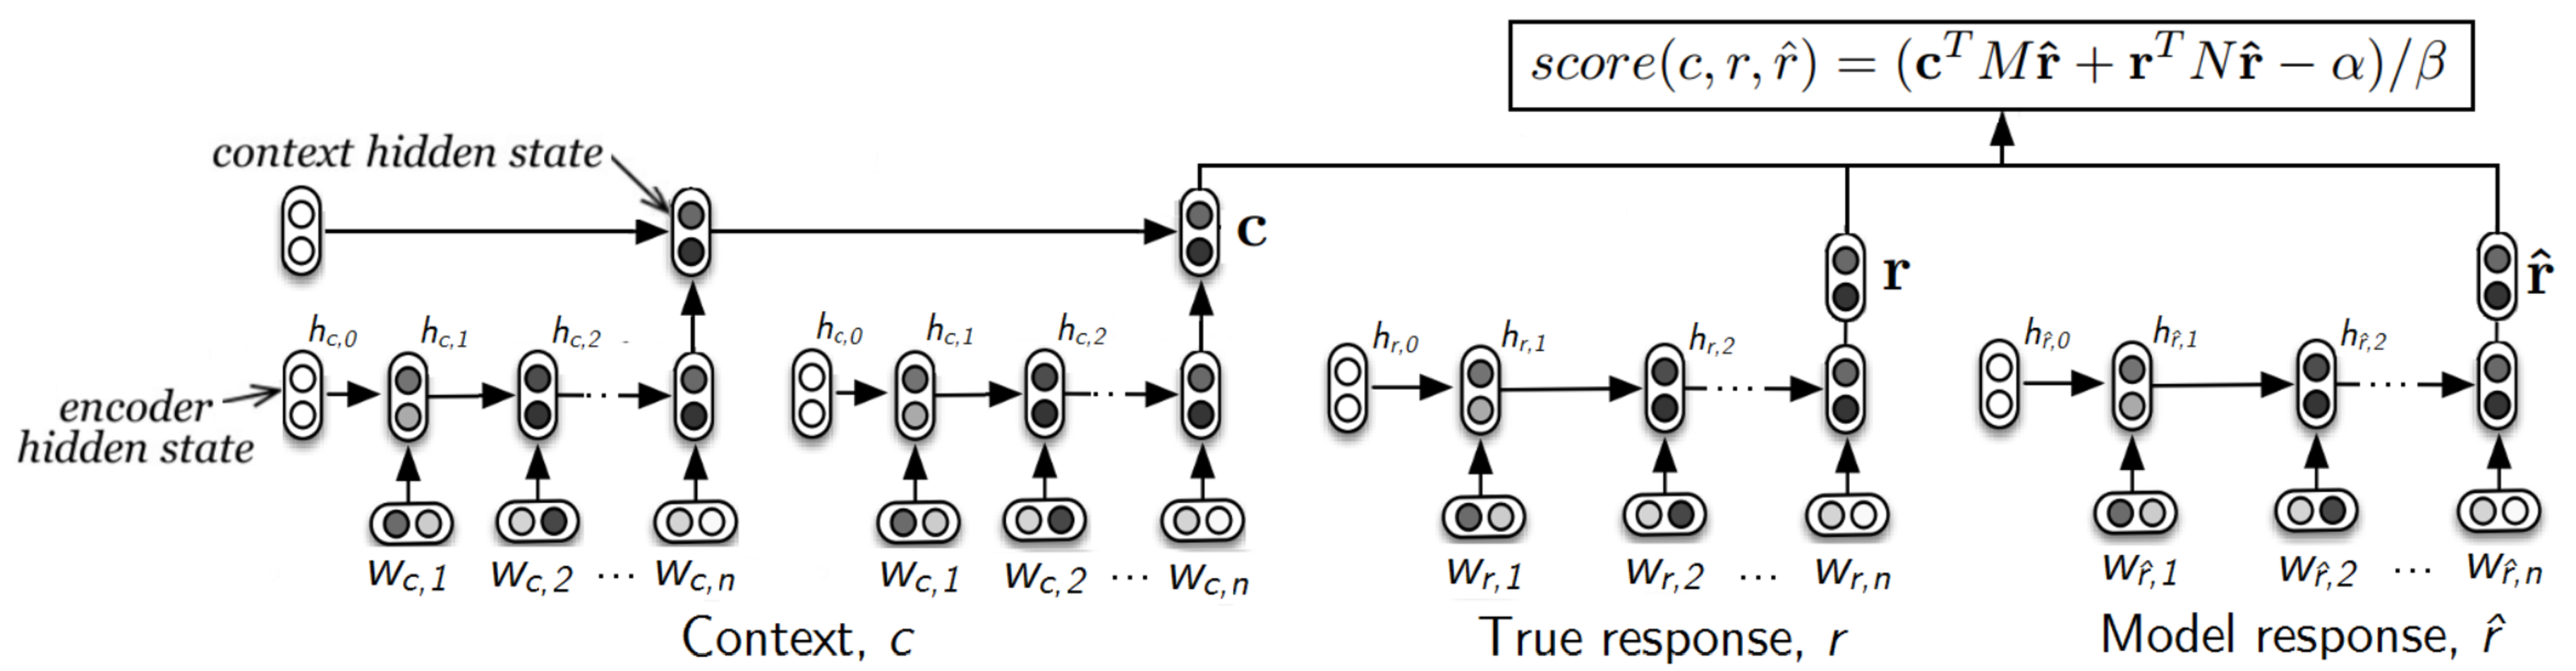
\includegraphics[width=0.9\textwidth]{figure/ADEM.pdf}
    \caption{ADEM模型结构图}
    \label{fig:ADEM_model}
\end{figure}

公式~\ref{eqn:ADEM_score}~是ADEM的打分公式,$M, N$是可学习的
参数矩阵,$\alpha, \beta$是缩放常量,使得分落在$[1, 5]$区间。
如公式~\ref{eqn:ADEM_objective}~所示,
模型的训练目标函数是一个带L2正则化的均方误差。
\begin{align}
    \textit{score}(c, r, \hat{r}) = (c^T M \hat{r} + r^T N \hat{r} - \alpha) / \beta
    \label{eqn:ADEM_score} \\
    \mathcal{L} = \sum_{i=1:K} [\textit{score}(c_i, r_i, \hat{r}_i) - \textit{human}_i]^2 + \gamma \left\| \theta \right\| _2
    \label{eqn:ADEM_objective}
\end{align}
ADEM在一个带人类评价的Twitter数据集上训练并评估,
它的打分和人类评价的相关性在句子水平和系统水平都达到了较高水平。

% ------ RUBER --------- %
Tao等人提出了带参考和无参考的混合指标
(Referenced Metric and Unreferenced Metric Blended Evaluation Routine,RUBER)\upcite{RUBER}。
如图~\ref{fig:RUBER_components}~所示,
RUBER由带参考的指标(Referenced Score)和无参考的指标(Unreferenced Score)两部分组成。
带参考的指标使用
基于词嵌入的最大-最小池化(Max-Min Pooling)作为句子向量,
衡量了消息和响应的相似度,公式如下:
\begin{align}
    v_{max}[i] = \max \{ w_1[i], w_2[i], \dots, w_n[i] \} \\
    v_{min}[i] = \min \{ w_1[i], w_2[i], \dots, w_n[i] \} \\
    v = [v_{max}; v_{min}] \\
    s_R(r, \hat{r}) = \cos(v_r, v_{\hat{r}}) =
    \frac{v_r^T v_{\hat{r}}}{\left\| v_r \right\| \cdot \left\| v_{\hat{r}} \right\|}
\end{align}

无参考的指标通过如图~\ref{fig:RUBER_unref_model}~所示的神经网络估计响应和消息的相关程度。
该模型用负采样(Negative Sampling)训练,不需要人类评价作为监督信号。
RUBER在中文数据集豆瓣\footnote{\url{http://www.douban.com}}上取得了较高的人类评价相关性。
\begin{figure}[H]
    \begin{subfigure}{0.45\linewidth}
        \centering
        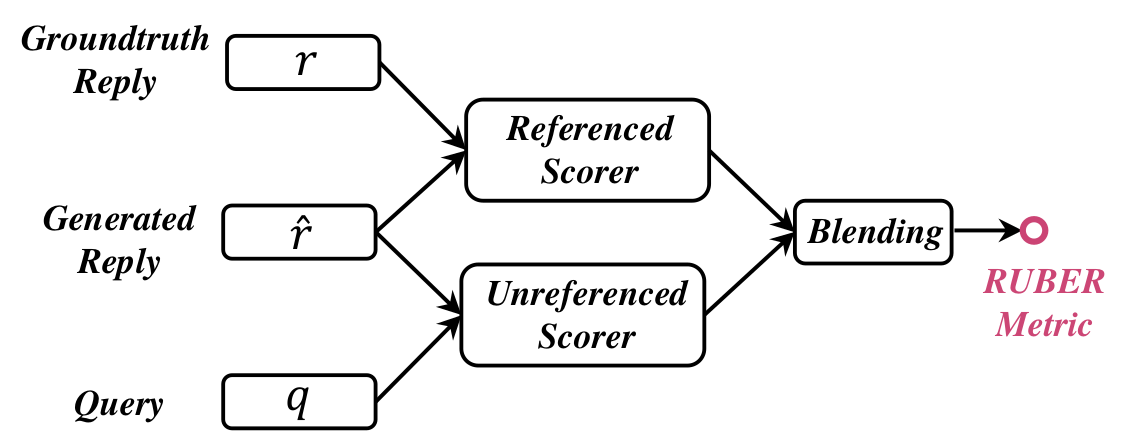
\includegraphics[width=\linewidth]{figure/RUBER_overview.png}
        \caption{RUBER的分数组成}
        \label{fig:RUBER_components}
    \end{subfigure}%
    \begin{subfigure}{0.45\linewidth}
        \centering
        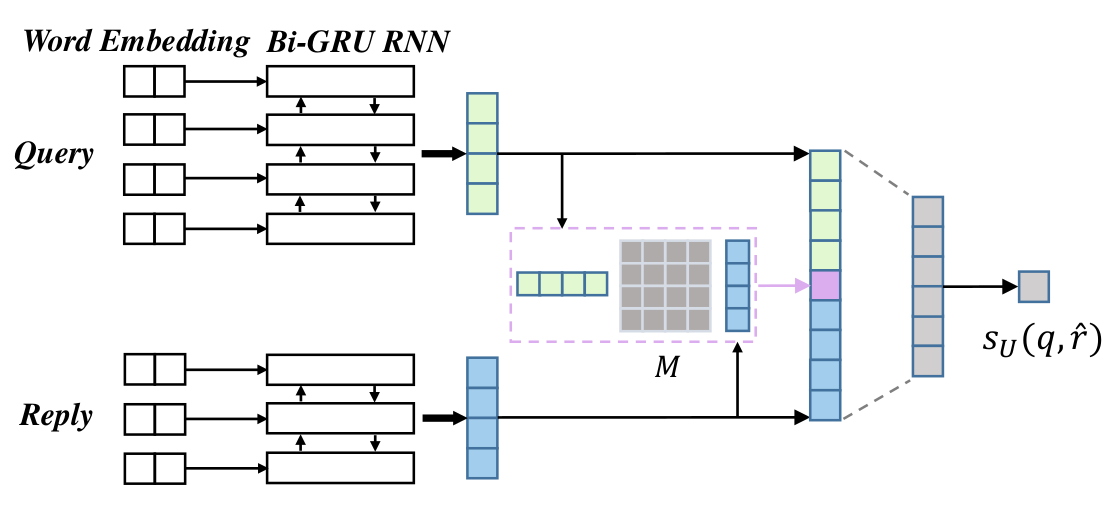
\includegraphics[width=\linewidth]{figure/RUBER_model.png}
        \caption{无参考指标的模型结构}
        \label{fig:RUBER_unref_model}
    \end{subfigure}
    \centering
    \caption{RUBER指标}
\end{figure}

% ------- AdverEval --------- %
Kannan等人初步尝试了基于对抗生成网络的对抗式评价
(Adversarial Evaluation)\upcite{AdverEval}。
他们训练了一个鉴别器(Discriminator)来区分一个响应是来自系统还是来自人类,
并且发现鉴别器能捕捉到基于Seq2Seq的模型倾向于生成短句子和通用句子的缺点。
基于相似的思路,Li等人在文献\cite{Adversarial}中构建了完整的对抗生成网络,
提出了训练和评价的一体框架。
关于对抗生成网络的内容超出了本文的范围,所以不再描述。

% -- Usage of Metrics -- %
\subsection{评价指标的使用情况}\label{subsec:metrics_usage}
生成式对话系统还没有公认的合适的评价指标。
学者们很早就意识到了这一点\upcite{Ritter11,GoogleChatbot,Shang,HRED},
所以他们常常使用人类评价作为核心的评判标准,有时用指标来衡量模型某一方面的特性,
但很少把指标作为评价系统的主要手段。
除了人类评价和指标,
展示并分析模型的输出也是衡量模型性能的常见方法,通常称为定性分析(Qualitative Analysis)。
表~\ref{tab:qualitative_analysis}~展示了模型GoogleChatbot对哲学问题的响应,
从中可以看出该模型对哲学问题的回答具有一定的语义相关性。
\begin{table}
    \centering
    \caption{定性分析的例子\upcite{GoogleChatbot}}
    \label{tab:qualitative_analysis}
    \begin{tabular}{ll}
        \toprule
        \midrule
        \textbf{人类:} & what is the purpose of life ? \\
        \textbf{模型:} & to serve the greater good .\\
        \midrule
        \textbf{人类:} & what is the purpose of living ? \\
        \textbf{模型:} & to live forever . \\
        \midrule
        \textbf{人类:} & what is the purpose of existence ? \\
        \textbf{模型:} & to find out what happens when we get to the planet earth . \\
        \midrule
        \textbf{人类:} & where are you now ? \\
        \textbf{模型:} & i' m in the middle of nowhere . \\
        \midrule
        \textbf{人类:} & what is the purpose of dying ? \\
        \textbf{模型:} & to have a life . \\
        \midrule
        \textbf{人类:} & what is the purpose of being intelligent ? \\
        \textbf{模型:} & to find out what it is . \\
        \midrule
        \textbf{人类:} & what is the purpose of emotions ? \\
        \textbf{模型:} & i don' t know . \\
        \bottomrule
    \end{tabular}
\end{table}

% Ritter -- MT-chat
Ritter等人首次尝试了数据驱动的,面向闲聊的对话响应生成\upcite{Ritter11}。
因为不清楚面向任务的指标能不能用于评价生成式模型,
他们就使用了亚马逊众包平台(Amazon Mechanical Turk,AMT)的人工评价。
他们利用人类评价的数据考察了BLEU在这方面的适用性,
并发现BLEU的系统层面得分非常低,和人类评价的相关性也不是很高。
据此他们认为BLEU不能直接应用到本领域。

% Shang -- NRM
Shang等人在评价他们的模型时分析了几种指标在本领域的适用性\upcite{Shang}。
他们认为BLEU并不适用,因为合理的响应的空间太大了,参考响应不可能完全覆盖到;
而常用于评价语言模型的困惑度也不适用,因为它不能测量响应的自然程度及其对消息的相关程度。
最后他们选择了人类评价。

% Sordoni -- DCGM-1-2
Sordoni在评价他们的模型时采用了BLEU和METEOR两种指标\upcite{DCGM}。
为了处理庞大而多样的响应空间,他们用信息检索(Information Retrieval,IR)的方法从数据集中挖掘潜在的合理响应,
并让人类评估员对其合适度(Appropriateness)打分,
从而构造了一个多重参考测评集(Multiple-Responses Benchmark Dataset)。
在这样的测评集上,他们发现BLEU对系统的排名和人类评价非常一致。
这种构建方法也见于LSDSCC\upcite{LSDSCC}的测试集的构造,
以及DeltaBLEU\upcite{deltaBLEU}指标的设计思路。

% Serban -- HRED
Serban等人在HRED模型的评价中使用了困惑度和单词分类错误(Word Classification Error,WCE)\upcite{HRED}。
他们认为困惑度是适用的,因为在存在多个合理输出的情况下,困惑度总是衡量生成单一参考输出的概率,
这意味着它能可靠的衡量模型的质量。
单词分类错误是模型的输出中正确预测的单词占整个数据集的单词的比例。
这里的“正确预测”要求单词在句子中的顺序也要正确,所以它比困惑度更严苛。
尽管使用了自动化指标,
Serban等人指出:这些指标与语法正确度(Grammatical Correctness)
和语义连贯度(Semantic Coherence)之间的相关性并不明确。
值得注意的是,他们并没有使用人类评价。

% Serban -- VHRED
Serban等人在VHRED模型的评价中使用了基于词嵌入的指标\upcite{VHRED}和人类评价。
他们认为,虽然基于词嵌入的指标和人类评价的相关度不高,
但是它们可以衡量话题相似性(Topic Similarity),
即模型的响应和参考之间的语义是否相似。
他们用人类评价和定性分析验证了基于词嵌入的指标所衡量的话题相似性。

% Vinyals -- Google Chatbot
Vinyals等人在评价他们的模型时使用了困惑度,定性分析和人类评价\upcite{GoogleChatbot}。
尽管他们的模型在上述评价中都打败了基线模型,
但是他们认为这些评价方法都存在许多弊端。
能快速并且准确的评价系统性能的指标仍有待学界研究。

% -- Dataset -- %
\section{开放领域的对话数据集}\label{sec:public_dataset}
本领域所使用的数据集一般称为开放领域的对话数据集(Open-Domain Dialogue Corpus)。
和传统的面向任务的数据集相比,它们的话题广泛,语法形式多样,
而且常带有非自然语言符号(表情符号,URL等等)\upcite{corpus_survey}。
表~\ref{tab:dataset_list}~列举了一些常见的数据集,
大规模是指样本数量在1M及以上的,
中等规模是指样本数量在50K--1M之间的\footnote{1K = 1024,1M = 1024 K,1G = 1024 M。}。
新浪微博数据集(Sina Weibo Corpus)是一个中文数据集,其他都是英文数据集。
与Twitter相关的数据集由于隐私保护政策的原因,不能公开原始数据。
数据集\upcite{supreme,wiki_pages,tennis_corpus,parliamentary,gone_awry,movie_dialogs_corpus,DailyDialog}都具有元信息,
如时间戳,对话双方身份信息等等。
数据集\upcite{DailyDialog,LSDSCC,DCGM}都有人类标注信息,
如情感、话题和方面(Aspect)等。
元信息和人类标注信息提供了额外的表征,对构建更智能的对话系统很有帮助。
本文把注意力集中在三个数据集上:
Ubuntu对话数据集(Ubuntu Dialogue Corpus),OpenSubtitles,
LSDSCC数据集(A Large Scale Domain-Specific Conversation Corpus),
它们代表了三个常见的对话领域:技术支持,电影字幕和在线论坛。
\begin{table}
    \centering
    \caption{开放领域的对话数据集}
    \label{tab:dataset_list}
    \begin{tabular}{llll}
        \toprule
        名称 & 规模 & 领域 & 是否公开 \\
        \midrule
        Ubuntu Dialogue Corpus\upcite{ubuntu_corpus} & 大 & 技术支持 & 是 \\
        Twitter Corpus\upcite{Ritter11} & 大 & 短文本多领域闲聊 & 否 \\
        Twitter Triple Corpus\upcite{DCGM} & 大 & Twitter Corpus的扩展版本 & 否 \\
        OpenSubtitles\upcite{OPUS,opensub} & 大 & 电影字幕(Subtitles) & 是 \\
        LSDSCC\upcite{LSDSCC} & 中 & Reddit论坛电影板块 & 是 \\
        Supreme Court Corpus\upcite{supreme} & 中 & 美国高等法院辩论 & 是\\
        Wikipedia Talk Pages Corpus\upcite{wiki_pages} & 中 & 维基百科编辑者在线讨论 & 是 \\
        Tennis Corpus\upcite{tennis_corpus} & 中 & 网球比赛赛后新闻发布会 & 是 \\
        Parliament Corpus\upcite{parliamentary} & 中 & 国会讨论 & 是 \\
        Conversations Gone Awry Corpus\upcite{gone_awry} & 中 & 维基百科讨论页面吵架集锦 & 是 \\
        Movie Dialogs Corpus\upcite{movie_dialogs_corpus} & 中 & 电影对白 & 是 \\
        Movie-DiC\upcite{Movie-DiC} & 中 & IMSDB电影对白 & 否 \\
        MovieTriples\upcite{HRED} & 中 & Movie-DiC的扩展版本 & 否 \\
        SubTle\upcite{Luke_SubTle} & 中 & 电影字幕 & 否 \\
        DailyDialog\upcite{DailyDialog} & 中 & 日常对话 & 是 \\
        Sina Weibo Corpus\upcite{weibo} & 中 & 新浪微博短文本闲聊 & 是 \\
        \bottomrule
    \end{tabular}
\end{table}

% --------- Ubuntu ---------- %
Ubuntu对话数据集(下文简称Ubuntu)
是Lowe等人从Freenode IRC网络的Ubuntu板块的聊天日志\footnote{\url{https://irclogs.ubuntu.com/}}
中获取的技术性两人多轮对话。
这个数据集包含了大量技术符号,比如路径,命令,URL,还有笔误(Typo),缩写(Abbreviation)和俚语(Slang)。
它的样本数量多达930,000(接近1M),庞大的数据量为数据驱动的模型提供了极佳的试验场。
它的多轮特性为模型提供了更长的上下文,有助于模型生成更有意义的响应。

% --------- OpenSubtitles -------- %
OpenSubtitles是开源双语数据集项目(The Open Parallel Corpus,OPUS)的一部分。
它是从一个人们可以自由上传和下载电影字幕的网站\footnote{\url{http://www.opensubtitles.org}}的数据库中获取的,
庞大而充满噪音的开放领域数据集,对话数量高达80M。
由于OPUS的目的是收集机器翻译所需要的双语数据集(Parallel Corpus),OpenSubtitles也是一个双语数据集,
它里面并没有对话数据集所需要的轮信息(Turn Information),
而且也没有区分旁白,独白和对白。
Sordoni等人把OpenSubtitles用到对话领域\upcite{GoogleChatbot},
他们把相邻的两个句子分别视为消息和响应,并且每一个句子既是消息又是响应。
Li等人对OpenSubtitles也采用了类似的办法\upcite{MMI,persona,Future,DiverseBeam,
Distill,deep_RL,Adversarial}。

% --------- LSDSCC ------------- %
大规模特定领域对话数据集(A Large Scale Domain-Specific Conversational Corpus,LSDSCC)
是一个特定领域的单轮对话数据集\upcite{LSDSCC}。
它的训练集包含738,095个样本;它的词汇表比较大,达到了50K。
作者从Reddit的电影板块\footnote{\url{https://www.reddit.com/r/datasets}}中获取原始数据,
设计了一套尽可能保留语料信息的清理程序,还使让人类评价员对消息和响应的相关度进行评价,
最终得到一个高质量的消息-响应对数据集(Query-Reply Pair Corpus)。
作者还用信息检索的方法构建了一个多重参考测评集,并基于此提出了一系列衡量响应多样性的指标。

% -- Conclusion -- %
% to be short? move to exp.
\section{本章小结}\label{sec:rw_conclusion}
本章从模型,指标和数据集三个方面回顾了本领域的研究现状。
在模型方面,基于Seq2Seq的对话系统有多种优势,例如:
能够直接生成响应,
能端对端的训练,
能从大量语料数据中自动学习语言规律,减少写死的规则,
能利用话题和情感等多种表征,等等。
然而这类系统也有弊端,
比如无法准确控制生成的内容,
偏向于生成单调的响应,
没有人格一致性等等。

在指标方面,对话系统的指标还不能像机器翻译的指标那样准确的评价系统的性能。
% -- this is totally disscusion.
目前最大的问题可能是如何提高指标和人类评价的相关性。
导致这个困境的核心原因可能是对话的响应具有固有的语义多样性,
这个事实可能导致两个结果:1. 用机器翻译的表征,比如单词层面的n-gram,字符层面的n-gram,
对齐等等,无法有效捕捉语义层面的信息。
2. 单纯使用衡量相似性的指标无法捕捉多样性的维度,从而与人类评价不符。

在数据集方面,本领域已经积累了来自不同领域的数据,例如技术性问答,社交媒体上的闲聊,电影对白和字幕,等等。
一些数据集在领域上出现了重合,
比如电影对话数据集(Movie Dialogs Corpus),
电影三元组数据集(MovieTriples)和Movie-DiC的领域都是电影对白;
OpenSubtitles和SubTle的领域都是电影字幕;
Twitter数据集(Twitter Corpus),
Twitter对话数据集和Twitter三元组数据集的领域都是Twitter短文本闲聊。
% -- This is totally future_work.
尽管人类标注是对话文本的重要补充,但是由于其代价的高昂,
所得的数据量往往比较少;
另一方面,元信息是一类在数据采集过程中伴随对话文本同时获得的描述性信息,
比如对话者的性别(Gender)和角色(Character)等等。
相比与人类标注,元信息更容易获取,规模不受限制。
并且,人类标注和元信息都有助于模型生成更加多样和连贯的响应
\upcite{persona,Topic_Aware,ECM}。
因此,数据集的收集过程应该充分保留原始数据中的元信息,
对话系统应该充分利用元信息。
同时,还应该发展从对话文本中无监督的提取元信息的方法。
